\begin{frame}{Contributions}\framesubtitle{TopicCoRank}
  Adaptation supervisée de TopicRank aux domaines de spécialité

  \vspace{1em}

  \begin{block}{Objectif}
    Réaliser conjointement extraction et assignement
  \end{block}

  \vspace{1em}

  \begin{block}{Hypothèses}
    \begin{itemize}
      \item{Les documents d'apprentissage représentent le domaine}
      \begin{itemize}
        \item{Termes-clés $\simeq$ vocabulaire du domaine}
        \item{Lien d'association entre les termes-clés d'un même document}
      \end{itemize}
      \item{Le domaine complète le document}
    \end{itemize}
  \end{block}
\end{frame}

\begin{frame}{TopicCoRank}\framesubtitle{TopicCoRank}
  \begin{block}{Propositions}
    \begin{itemize}
      \item{Représentation du domaine par un graphe}
      \item{Unification du graphe du domaine au graphe de sujets}
      \item{Ordonnancement conjoint}
    \end{itemize}
  \end{block}
\end{frame}

\begin{frame}{TopicCoRank}\framesubtitle{Aperçu}
  Phases préparatoires de TopicRank~:
  \begin{enumerate}
    \item{Sélection des termes-clés candidats du document}
    \item{Groupement des candidats en sujets}
    \item{Création du graphe de sujets}
  \end{enumerate}
  \vspace{.25em}\hrule\vspace{.5em}
  Ajout de la connaissance du domaine~:
  \begin{enumerate}
    \setcounter{enumi}{3}
    \item{Déduction du vocabulaire contrôlé du domaine}
    \item{Création du graphe des termes-clés du domaine}
    \item{Unification du graphe du domaine au graphe de sujets}
  \end{enumerate}
  \vspace{.25em}\hrule\vspace{.5em}
  Extraction et assignement conjoints~:
  \begin{enumerate}
    \setcounter{enumi}{6}
    \item{Ordonnancement conjoint des sujets et des termes-clés du domaine}
    \item{Sélection des termes-clés parmi les meilleurs sujets et/ou termes-clés
          du domaine}
  \end{enumerate}
\end{frame}

\begin{frame}{TopicCoRank}\framesubtitle{Exemple}
  \vspace{-.33em}
  \alt<2->{
    \begin{exampleblock}{\small
      \underline{Étude préliminaire} de la \textbf{\underline{céramique} non
      tournée} \textbf{micacée} du \underline{bas Languedoc occidental}~:
      \textbf{\underline{typologie}}, \textbf{\underline{chronologie}} et
      \underline{aire} de \textbf{\underline{diffusion}}
    }\justifying\small
    ~~~L'\underline{étude} présente une \underline{variété} de
      \textbf{\underline{céramique} non tournée} dont la
      \textbf{\underline{typologie}} et l'\underline{analyse} des
      \textbf{\underline{décors}} permettent de l'identifier facilement. La
      \underline{nature} de l'\underline{argile} \underline{enrichie} de \underline{mica}
      donne un \underline{aspect} pailleté à la \underline{pâte} sur laquelle
      le \textbf{\underline{décor}} effectué selon la \underline{méthode} du
      \underline{brunissoir} apparaît en \underline{traits} brillant sur
      \underline{fond mat}. Cette \underline{première approche} se fonde sur
      deux \underline{séries issues} de \textbf{\underline{fouilles
      anciennes}} menées sur les \textbf{\underline{oppidums}} \textbf{du
      \underline{Cayla}} à \textbf{\underline{Mailhac}}
      (\textbf{\underline{Aude}}) et de \textbf{\underline{Mourrel-Ferrat}} à
      \textbf{\underline{Olonzac}} (\textbf{\underline{Hérault}}). La
      \underline{carte} de \textbf{\underline{répartition}} fait
      \underline{état} d'\textbf{\underline{échanges}} ou de
      \textbf{\underline{commerce}} à l'\underline{échelon macrorégional}
      rarement mis en \underline{évidence} pour de la
      \textbf{\underline{céramique} non tournée}. S'il est \underline{difficile}
      de statuer sur l'\underline{origine} des \textbf{\underline{décors}}, il
      semble que la \textbf{\underline{production}} s'insère dans une
      \underline{ambiance celtisante}. La \textbf{\underline{chronologie}} de
      cette \textbf{\underline{produ-} \underline{ction}} se situe dans le \underline{deuxième
      \textbf{âge}} \textbf{du Fer}. La \underline{fourchette} proposée entre la
      \underline{fin} du \underline{IV$^\text{e}$} et la \underline{fin} du
      II$^\text{e}$ s. av. \underline{J.-C.} reste encore à préciser.

      \begin{exampleblock}{\small Termes-clés de référence}\justifying\small
        \textbf{Mailhac}~; \textbf{Aude}~; \textbf{Mourrel-Ferrat}~;
        \textbf{Olonzac}~; \textbf{Hérault}~; \textbf{céramique}~;
        \textbf{typologie}~; \textbf{décor}~; \textbf{chronologie}~;
        \textbf{diffusion}~; \textbf{production}~; \textbf{commerce}~;
        \textbf{répartition}~; \textbf{oppidum}~; \textbf{analyse}~;
        \textbf{fouille ancienne}~; \textbf{le Cayla}~;
        \textbf{micassé}~; \textbf{céramique non-tournée}~;
        \textbf{echange}~; \textbf{age du} \textbf{Fer}~; La Tène~;
        Europe~; France~; celtes~; distribution~; cartographie~; habitat~; site
        fortifié~; identification~; étude du matériel
      \end{exampleblock}
    \end{exampleblock}
  }{
    \begin{exampleblock}{\small
      Étude préliminaire de la \textbf{céramique non tournée}
      \textbf{micacée} du bas Languedoc occidental~: \textbf{typologie},
      \textbf{chronologie} et aire de \textbf{diffusion}
    }\justifying\small
      ~~~L'étude présente une variété de \textbf{céramique non tournée} dont la
      \textbf{typologie} et l'analyse des \textbf{décors} permettent de
      l'identifier facilement. La nature de l'argile enrichie de mica donne un
      aspect pailleté à la pâte sur laquelle le \textbf{décor} effectué selon
      la méthode du brunissoir apparaît en traits brillant sur fond mat. Cette
      première approche se fonde sur deux séries issues de \textbf{fouilles
      anciennes} menées sur les \textbf{oppidums} \textbf{du Cayla} à
      \textbf{Mailhac} (\textbf{Aude}) et de \textbf{Mourrel-Ferrat} à
      \textbf{Olonzac} (\textbf{Hérault}). La carte de
      \textbf{répartition} fait état d'\textbf{échanges} ou de
      \textbf{commerce} à l'échelon macrorégional rarement mis en évidence pour
      de la \textbf{céramique non tournée}. S'il est difficile de statuer sur
      l'origine des \textbf{décors}, il semble que la \textbf{production}
      s'insère dans une ambiance celtisante. La \textbf{chronologie} de cette
      \textbf{production} se situe dans le deuxième \textbf{âge du Fer}. La
      fourchette proposée entre la fin du IV$^\text{e}$ et la fin du II$^\text{e}$
      s. av. J.-C. reste encore à préciser.

      \begin{exampleblock}{\small Termes-clés de référence}\justifying\small
        \textbf{Mailhac}~; \textbf{Aude}~; \textbf{Mourrel-Ferrat}~;
        \textbf{Olonzac}~; \textbf{Hérault}~; \textbf{céramique}~;
        \textbf{typologie}~; \textbf{décor}~; \textbf{chronologie}~;
        \textbf{diffusion}~; \textbf{production}~; \textbf{commerce}~;
        \textbf{répartition}~; \textbf{oppidum}~; \textbf{analyse}~;
        \textbf{fouille ancienne}~; \textbf{le Cayla}~;
        \textbf{micassé}~; \textbf{céramique non-tournée}~;
        \textbf{echange}~; \textbf{age du} \textbf{Fer}~; La Tène~;
        Europe~; France~; celtes~; distribution~; cartographie~; habitat~; site
        fortifié~; identification~; étude du matériel
      \end{exampleblock}
    \end{exampleblock}
  }
\end{frame}

\begin{frame}[label=ordonnancement_conjoint_back]{TopicCoRank}\framesubtitle{\hyperlink{ordonnancement_conjoint}{Exemple}}
  \newcommand{\xslant}{0.25}
  \newcommand{\yslant}{0}
  \centering
  \begin{tikzpicture}[transform shape, scale=.75]
    % frames %%%%%%%%%%%%%%%%%%%%%%%%%%%%%%%%%%%%%%%%%%%%%%%%%%%%%%%%%%%%%%%%%%%
    \uncover<1->{
      \node [draw,
             rectangle,
             minimum width=1.15\linewidth,
             minimum height=.5\textheight,
             xslant=\xslant,
             yslant=\yslant] (domain_graph) {};
    }
    \uncover<3->{
      \node [draw,
            rectangle,
            minimum width=1.15\linewidth,
            minimum height=.5\textheight,
            xslant=\xslant,
            yslant=\yslant,
            above=of domain_graph,
            xshift=-3.5em] (document_graph) {};
    }

    % domain %%%%%%%%%%%%%%%%%%%%%%%%%%%%%%%%%%%%%%%%%%%%%%%%%%%%%%%%%%%%%%%%%%%
    \uncover<3->{
      \node [above=of domain_graph,
             xshift=.575\linewidth,
             yshift=.5\textheight,
             anchor=south east] (domain_graph_label) {termes-clés du domaine (sous-partie)};

      % nodes
      \node [above=of domain_graph,%draw,
             xshift=-1.9em,
             yshift=.425\textheight] (france) {\alt<6->{\textcolor{termithorange}{\textbf{France}}}{France}};
      \node [above=of domain_graph,%draw,
             xshift=-7.5em,
             yshift=.29\textheight] (typologie) {typologie};
      \node [above=of domain_graph,%draw,
             xshift=4.3em,
             yshift=.29\textheight] (chronologie) {chronologie};
      \node [above=of domain_graph,%draw,
             xshift=-16.5em,
             yshift=.22\textheight] (ceramique) {céramique};
      \node [above=of domain_graph,%draw,
             xshift=13em,
             yshift=.22\textheight] (production) {production};
      \node [above=of domain_graph,%draw,
             xshift=2.2em,
             yshift=.1\textheight] (analyse) {\alt<6->{\textcolor{termithorange}{\textbf{analyse}}}{analyse}};
      \node [above=of domain_graph,%draw,
             xshift=-5.2em,
             yshift=.1\textheight] (decor) {décor};
      \node [above=of domain_graph,%draw,
             xshift=-12.5em,
             yshift=.01\textheight] (repartition) {répartition};
      \node [above=of domain_graph,%draw,
             xshift=9.5em,
             yshift=.02\textheight] (diffusion) {diffusion};
    }

    \uncover<4->{
      % france
      \draw (france) -- (typologie);
      \draw (france) -- (chronologie);
      \draw (france) -- (production);
      \draw (france) -- (diffusion);
      \draw (france) -- (decor);
      \draw (france) -- (analyse);
      \draw (france) -- (repartition);
      \draw (france) -- (ceramique);
      % typologie
      \draw (typologie) -- (chronologie);
      \draw (typologie) -- (production);
      \draw (typologie) -- (diffusion);
      \draw (typologie) -- (decor);
      \draw (typologie) -- (analyse);
      \draw (typologie) -- (repartition);
      \draw (typologie) -- (ceramique);
      % chronologie
      \draw (chronologie) -- (production);
      \draw (chronologie) -- (diffusion);
      \draw (chronologie) -- (decor);
      \draw (chronologie) -- (analyse);
      \draw (chronologie) -- (repartition);
      \draw (chronologie) -- (ceramique);
      % production
      \draw (production) -- (diffusion);
      \draw (production) -- (decor);
      \draw (production) -- (analyse);
      \draw (production) -- (ceramique);
      % diffusion
      \draw (diffusion) -- (decor);
      \draw (diffusion) -- (analyse);
      \draw (diffusion) -- (ceramique);
      % decor
      \draw (decor) -- (analyse);
      \draw (decor) -- (ceramique);
      % analyse
      \draw (analyse) -- (ceramique);
    }

    % document %%%%%%%%%%%%%%%%%%%%%%%%%%%%%%%%%%%%%%%%%%%%%%%%%%%%%%%%%%%%%%%%%
    \uncover<1->{
      \node [below=of document_graph,
             xshift=-.575\linewidth,
             yshift=-.5\textheight,
             anchor=north west] (document_graph_label) {sujets du document (sous-partie)};

      \node [minimum width=2.5em,
             below=of document_graph,%draw,
             xshift=-4em,
             yshift=-.05\textheight] (typologie_c) {\alt<6->{\textcolor{termithorange}{\textbf{[typologie]}}}{[typologie]}};
      \node [minimum width=2.5em,
             below=of document_graph,%draw,
             xshift=10.75em,
             yshift=-.05\textheight] (chronologie_c) {\alt<6->{\textcolor{termithorange}{\textbf{[chronologie]}}}{[chronologie]}};
      \node [minimum width=2.5em,
             below=of document_graph,%draw,
             xshift=-13.1em,
           yshift=-.25\textheight] (ceramique_c) {\alt<6->{\textcolor{termithorange}{\textbf{[céramique]}}}{[céramique]}};
      \node [minimum width=2.5em,
             below=of document_graph,%draw,
             xshift=17em,
             yshift=-.125\textheight] (production_c) {\alt<6->{\textcolor{termithorange}{\textbf{[production]}}}{[production]}};
      \node [minimum width=2.5em,
             below=of document_graph,%draw,
             xshift=2.5em,
             yshift=-.25\textheight] (analyse_c) {[analyse]};
      \node [minimum width=2.5em,
             below=of document_graph,%draw,
             xshift=.5em,
             yshift=-.40\textheight] (decor_c) {\alt<6->{\textcolor{termithorange}{\textbf{[décors~; décor]}}}{[décors~; décor]}};
      \node [minimum width=2.5em,
             below=of document_graph,%draw,
             xshift=-9em,
             yshift=-.40\textheight] (repartition_c) {\alt<6->{\textcolor{termithorange}{\textbf{[répartition]}}}{[répartition]}};
      \node [minimum width=2.5em,
             below=of document_graph,%draw,
             xshift=15em,
             yshift=-.40\textheight] (diffusion_c) {\alt<6->{\textcolor{termithorange}{\textbf{[diffusion]}}}{[diffusion]}};
      \node [minimum width=2.5em,
             below=of document_graph,%draw,
             xshift=7.66em,
             yshift=-.16\textheight] (etude_preliminaire_c) {\alt<6->{\textcolor{termithorange}{\textbf{[étude préliminaire]}}}{[étude préliminaire]}};
      \node [minimum width=2.5em,
             below=of document_graph,%draw,
             xshift=17em,
             yshift=-.25\textheight] (fer_c) {[fer]};
    }

    \uncover<2->{
      % typologie
      \draw (typologie_c) -- (chronologie_c);
      \draw (typologie_c) -- (diffusion_c);
      \draw (typologie_c) -- (decor_c);
      \draw (typologie_c) -- (analyse_c);
      \draw (typologie_c) -- (ceramique_c);
      % chronologie
      \draw (chronologie_c) -- (production_c);
      \draw (chronologie_c) -- (diffusion_c);
      \draw (chronologie_c) -- (ceramique_c);
      % production
      \draw (production_c) -- (decor_c);
      % diffusion
      \draw (diffusion_c) -- (ceramique_c);
      % decor
      \draw (decor_c) -- (analyse_c);
      \draw (decor_c) -- (repartition_c);
      \draw (decor_c) -- (ceramique_c);
      % analyse
      \draw (analyse_c) -- (ceramique_c);
      % répartition
      \draw (repartition_c) -- (ceramique_c);
      % étude préliminaire
      \draw (etude_preliminaire_c) -- (ceramique_c);
      \draw (etude_preliminaire_c) -- (chronologie_c);
      \draw (etude_preliminaire_c) -- (typologie_c);
      \draw (etude_preliminaire_c) -- (diffusion_c);
      % fer
      \draw (fer_c) -- (chronologie_c);
      \draw (fer_c) -- (production_c);
    }

    % extra link %%%%%%%%%%%%%%%%%%%%%%%%%%%%%%%%%%%%%%%%%%%%%%%%%%%%%%%%%%%%%%%
    \uncover<5->{
      \draw [dashed] (typologie) -- (typologie_c);
      \draw [dashed] (chronologie) -- (chronologie_c);
      \draw [dashed] (ceramique) -- (ceramique_c);
      \draw [dashed] (production) -- (production_c);
      \draw [dashed] (analyse) -- (analyse_c);
      \draw [dashed] (decor) -- (decor_c);
      \draw [dashed] (repartition) -- (repartition_c);
      \draw [dashed] (diffusion) -- (diffusion_c);
    }
  \end{tikzpicture}
\end{frame}

\begin{frame}{TopicCoRank}\framesubtitle{Exemple}
  \begin{table}
      \centering
      \begin{tabular}{r|l|l}
        \toprule
        \textbf{Rang} & \multicolumn{1}{c|}{\textbf{TopicRank}} & \multicolumn{1}{c}{\textbf{TopicCoRank}} \\
        \hline
        01 & \cellcolor{termithgreen!30}{décors} & \cellcolor{termithgreen!30}{céramique} \\
        02 & \cellcolor{termithgreen!30}{céramique} & \cellcolor{termithgreen!30}{décors} \\
        03 & \cellcolor{termithgreen!30}{chronologie} & \cellcolor{termithgreen!30}{typologie} \\
        04 & \cellcolor{termithgreen!30}{typologie} & \cellcolor{termithgreen!30}{chronologie} \\
        05 & \cellcolor{termithgreen!30}{production} & \cellcolor{termithgreen!30}{production} \\
        06 & fin & étude préliminaire \\
        07 & étude préliminaire & \cellcolor{termithgreen!30}{diffusion} \\
        08 & fer & \cellcolor{termithgreen!30}{analyse\hspace{4em}*} \\
        09 & deuxième âge & \cellcolor{termithgreen!30}{France\hspace{3.725em}**} \\
        10 & aire & \cellcolor{termithgreen!30}{répartition} \\
        \bottomrule
      \end{tabular}

      \caption{Termes-clés}
    \end{table}

    \vspace{-.75em}

    \begin{exampleblock}{\small Termes-clés de référence}\justifying\small
      \textbf{Mailhac}~; \textbf{Aude}~; \textbf{Mourrel-Ferrat}~;
      \textbf{Olonzac}~; \textbf{Hérault}~; \textbf{céramique}~;
      \textbf{typologie}~; \textbf{décor}~; \textbf{chronologie}~;
      \textbf{diffusion}~; \textbf{production}~; \textbf{commerce}~;
      \textbf{répartition}~; \textbf{oppidum}~; \textbf{analyse}~;
      \textbf{fouille ancienne}~; \textbf{le Cayla}~;
      \textbf{micassé}~; \textbf{céramique non-tournée}~;
      \textbf{echange}~; \textbf{age du} \textbf{Fer}~; La Tène~;
      Europe~; France~; celtes~; distribution~; cartographie~; habitat~; site
      fortifié~; identification~; étude du matériel
    \end{exampleblock}
%    \begin{block}{Observations}
%      \begin{itemize}
%        \item{Amélioration de l'ordonnancement grâce au domaine}
%        \item{Assignement de \og{}France\fg{} (hors document)}
%      \end{itemize}
%    \end{block}
\end{frame}

\begin{frame}{TopicCoRank}\framesubtitle{Évaluation}
    Trois méthodes de référence~:
    \begin{itemize}
      \item{TF-IDF~\cite{salton1975tfidf}}
      \item{TopicRank~\cite{bougouin2013topicrank}}
      \item{KEA++~\cite{medelyan2006kea++}}
    \end{itemize}

    \vspace{1em}

    Deux variantes~:
    \begin{itemize}
      \item{TopicCoRank$_\text{extr.}$}
      \item{TopicCoRank$_\text{assign.}$}
    \end{itemize}

    \begin{textblock*}{.4\textwidth}(.625\textwidth, -.275\textheight)
      \centering
      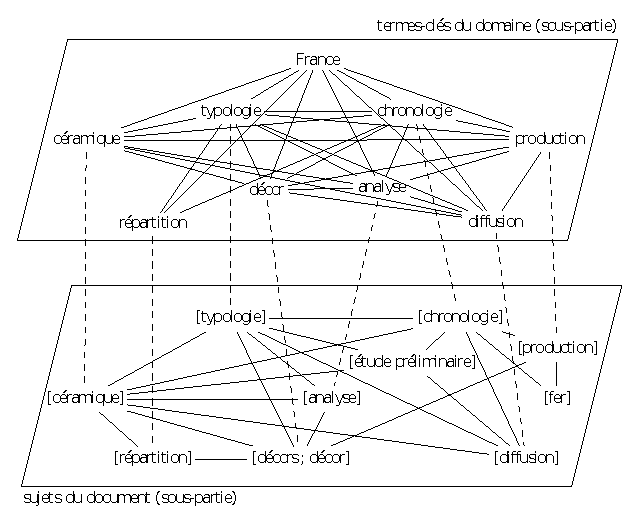
\includegraphics[width=\textwidth]{include/topiccorank_graph.eps}
    \end{textblock*}
\end{frame}

\begin{frame}[label=phrase_comme_contexte_back]{TopicCoRank}\framesubtitle{\hyperlink{phrase_comme_contexte}{Résultats}}
  \begin{table}
    \resizebox{\linewidth}{!}{
      \begin{tabular}{@{~}l|c@{~~}c@{~~}c@{~}|c@{~~~~~~~~}c@{~~~~~~}c@{~}|c@{~~}c@{~~}c@{~}|c@{~~}c@{~~}c@{~}}
        \toprule
        \multirow{2}{*}{\textbf{Méthode}} & \multicolumn{3}{c|}{\textbf{Linguistique} \textit{(fr)}} & \multicolumn{3}{c|}{\textbf{Sciences de l'info.} \textit{(fr)}} & \multicolumn{3}{c|}{\textbf{Archéologie} \textit{(fr)}} & \multicolumn{3}{c}{\textbf{Chimie} \textit{(fr)}}\\
        \cline{2-13}
        & P & R & F & P & R & F & P & R & F & P & R & F\\
        \hline
        \textsc{Tf-Idf} & 13,0 & 15,4 & 13,9 & 13,4 & 14,0 & 13,2$^{~}$ & 28,1 & 19,1 & 22,2$^{~~}$ & 14,1 & 11,1 & 11,9$^{~~}$\\
        TopicRank & 11,2 & 13,1 & 11,9 & 12,1 & 12,8 & 12,1$^{~}$ & 27,5 & 18,7 & 21,8$^{~~}$ & 13,8 & 11,1 & 11,8$^{~~}$\\
        KEA++ & 11,6 & 13,0 & 12,1 & $~~$9,5 & 10,2 & $~~$9,6$^{~~}$ & 23,5 & 16,2 & 18,8$^{~~}$ & 11,4 & $~~$8,5 & $~~$9,2$^{~~}$\\
        \hline
        TopicCoRank$_\textnormal{extr.}$ & 14,3 & 16,5 & 15,1 & 15,4 & 15,9 & 15,2$^\dagger$ & 36,7 & 24,6 & 28,8$^\dagger$ & 15,8 & 12,1 & 13,1$^{~~}$\\
        TopicCoRank$_\textnormal{assign.}$ & \textbf{24,5} & \textbf{28,3} & \textbf{25,8} & \textbf{19,7} & \textbf{19,8} & \textbf{19,2}$^\dagger$ & \textbf{47,8} & \textbf{32,3} & \textbf{37,7}$^\dagger$ & \textbf{20,0} & \textbf{14,8} & \textbf{16,3}$^\dagger$\\
        \hline
        TopicCoRank & 18,8 & 21,9 & 19,9 & 17,3 & 17,7 & 17,0$^\dagger$ & 38,3 & 25,7 & 30,1$^\dagger$ & 17,2 & 13,4 & 14,4$^\dagger$\\
        \bottomrule
      \end{tabular}
    }
  \end{table}

  \vspace{1em}

  \begin{block}{Observations}
    \begin{itemize}
      \item{Meilleure performance}
      \item{TopicCoRank$_\text{extr.}$ $>$ TopicRank $\Rightarrow$ apport du
            domaine}
    \end{itemize}
  \end{block}
\end{frame}

\begin{frame}{TopicCoRank}\framesubtitle{Bilan}
  Extension supervisée de TopicRank pour assigner des termes-clés

  \vspace{1em}

  \begin{block}{Avantages}
    \begin{itemize}
      \item{Tire profit de la connaissance du domaine}
      \item{Combine extraction et assignement $\Rightarrow$ meilleure
            exhaustivité}
      \item{Adapté à plusieurs scénarii d'utilisation professionnels~:}
      \begin{itemize}
        \item{TopicCoRank + validation~/~enrichissement manuel}
        \item{TopicCoRank$_\text{assign.}$ seul}
      \end{itemize}
    \end{itemize}
  \end{block}

  \vspace{1em}

  \begin{alertblock}{Limites}
    \begin{itemize}
      \item{Donne autant d'importance aux deux graphes}
      \item{Termes-clés extraits plus redondants que ceux de TopicRank}
    \end{itemize}
  \end{alertblock}
\end{frame}

